\documentclass[12pt]{article}
\usepackage{amsmath}
\usepackage{amssymb}
\usepackage{graphicx}
\usepackage{hyperref}
\usepackage[latin1]{inputenc}
\usepackage{listings}
\usepackage{pgfplots}
\renewcommand{\labelitemi}{$\textendash$}
\renewcommand{\arraystretch}{1.4}

\title{ST3009: Week 8 Assignment}
\author{Conor McCauley - 17323203}
\date{March 9, 2020}

\begin{document}

\maketitle

\section*{Question 1}

\noindent (a) Only a fraction of students will respond so there may be a bias in the results. Responses may not be entirely honest as many people might not want to admit that they are ``studying to pass".

\noindent (b) The random experiment that can be repeated many times in this case is the is individual response to the poll $X_i \in \{0, 1\}$. This relates to the issues outlined in part (a) in that, through only a fraction of people responding, we do not garner accurate results.

\indent A better way to design the experiment would be to make poll responses mandatory so that every student is sampled thus improving the overall accuracy of $Y$. Anonymous responses could be allowed in order to facilitate more honest responses.

\section*{Question 2}

\noindent (a) Two Bernoulli random variables, $X$ and $Y$, are identically distributed if and only if the cumulative distribution functions of $X$ and $Y$ are equal for every value of $x \in \mathbb{R}$:

$$ P(X \leq x) = P(Y \leq x) \indent \forall x \in \mathbb{R} $$

\indent Using the standard definition of independence for two events $E$ and $F$, $P(E \cap F) = P(E) \cdot P(F)$, we know that two Bernoulli random variables, $X$ and $Y$, are independent if and only if:

$$ P(X \leq x \cap Y \leq y) = P(X \leq x) \cdot P(Y \leq y) \indent \forall x, y \in \mathbb{R} $$

\noindent (b) Since each $X_i$ has $\mu = 0.1$ we know that $P(X_i = 1) = 0.1$ for all $i$. Thus

$$ Y = \frac{1}{N}\sum_{i = 1}^N X_i = \frac{1}{N} (X_i \cdot N) = X_i $$

\indent $Y$ is the empirical mean and, given that each $X_i$ is a random variable and since $Y = X_i$, we know that $Y$ is also a random variable. The mean of $Y$ is the same as the mean of any $X_i$ which is $0.1$.

\indent We can find the variance of $Y$ like so:

$$ Var(Y) = Var(\frac{1}{N}\sum_{i = 1}^N X_i) = \frac{1}{N^2} \sum_{i = 1}^N Var(X_i) = \frac{1}{N} Var(X_i) $$

\indent First we must calculate $Var(X_i)$:

$$ Var(X_i) = E[{X_i}^2] - E[{X_i}]^2 $$
$$ = \left( P(X_i = 1) \cdot 1^2 + P(X_i = 0 ) \cdot 0^2 \right) - (0.1)^2 $$
$$ = (0.1 \cdot 1^2 + 0.9 \cdot 0^2) - (0.01) $$
$$ = 0.09 $$

\indent Therefore, given $N = 100$:

$$ Var(Y) = \frac{0.09}{100}. = 0.0009 $$

\noindent (c) Given $N = 100$, $\mu = 0.1$ and $\sigma = \sqrt{0.0009} = 0.03$ we can calculate the 95\% confidence interval using Chebyshev's inequality like so:

$$ 0.1 - \frac{0.03}{\sqrt{0.05 \cdot 100}} \leq Y \leq 0.1 + \frac{0.03}{\sqrt{0.05 \cdot 100}} $$
$$ 0.1 - 0.0134 \leq Y \leq 0.1 + 0.0134 $$
$$ 0.0866 \leq Y \leq 0.1134 $$

\noindent (d) Again, given $N = 100$, $\mu = 0.1$ and $\sigma = 0.03$ we can calculate the 95\% confidence interval ($2\sigma$) using the CLT like so:

$$ 0.1 - 2 \cdot \frac{0.03}{\sqrt{100}} \leq Y \leq 0.1 + 2 \cdot \frac{0.03}{\sqrt{100}} $$
$$ 0.1 - 0.006 \leq Y \leq 0.1 + 0.006 $$
$$ 0.094 \leq Y \leq 0.106 $$

\indent We can see that the CLT gave us a tighter approximate bound than Chebyshev's inequality. However, one of the drawbacks of CLT is that it only provides an approximation related to the finite value of $N$. Chebyshev's inequality provided us with an actual bound which works for any value of $N$ but it is looser than CLT.

\noindent (e) Using the following code we can run the numerical simulation 10,000 times and estimate the PMF and 95\% confidence interval:

\begin{lstlisting}[language=Matlab]
    S = 10000;       % number of simulations to run
    N = 100;         % number of BRVs to generate
    R = zeros(S, 1); % simulation results
    M = 0.1;         % mean of Y
    
    % run simulations
    for s = 1:S
        R(s) = sum((rand(1, N) < M)) / N; % store empirical mean
    end
    
    % plot data
    [n, es] = histcounts(R, N, 'Normalization','probability');
    es = es(2:end) - (es(2) - es(1)) / 2;
    plot(es, n);
    
    % plot settings
    axis([0 1 0 1]);
    xticks(0:0.1:1);
    yticks(0:0.1:1);
    xlabel('Empirical Mean');
    ylabel('Probability');
    
    % estimate 95% CI
    m = mean(R);
    sd = std(R);
    chebLower = m - (sd / sqrt(N * 0.05));
    chebUpper = m + (sd / sqrt(N * 0.05));
    cltLower = m - (2 * (sd / sqrt(N)));
    cltUpper = m + (2 * (sd / sqrt(N)));
    
    fprintf("Chebyshev: %.5f <= Y <= %.5f \n", chebLower, chebUpper);
    fprintf("CLT:       %.5f <= Y <= %.5f \n", cltLower, cltUpper);
\end{lstlisting}

\indent This produces the following probability mass function:

\begin{center}
    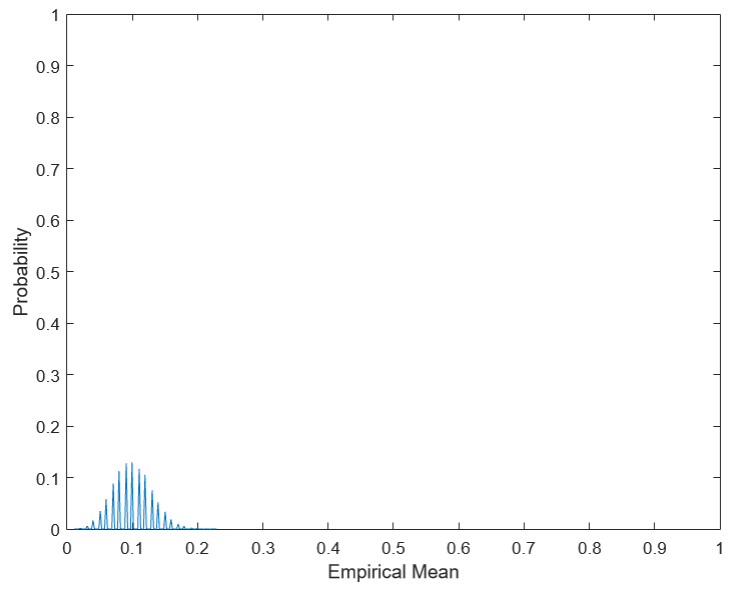
\includegraphics[scale=0.7]{plot.png}
\end{center}

\indent It also produces the following estimate for the 95\% confidence interval:

\begin{center}
    \indent Chebyshev: $0.08656 \le Y \le 0.11323$ 

    \indent CLT: $0.09393 \le Y \le 0.10585$
\end{center}

\indent The answers given in (c) and (d) are almost identical to their respective simulated results which tells us that the simulation is extremely accurate when run 10,000 times.

\end{document}
